\section{Beispiele}
Diese Beispiele wurden in einer dafür konzipierten Erweiterung für das \name{mec2} HTML Element gezeichnet.
Komplexere Skizzen von Mechanismen in einem Durchgang zu erkennen, ist mit den aktuellen Modellen noch mühselig.
Die Modelle müssten vorab für den genutzten Anwendungsbereich trainiert werden, um die korrekte Funktionsweise zu gewährleisten.

\begin{figure}[H]
    \centering
    \begin{subfigure}[b]{0.3\textwidth}
        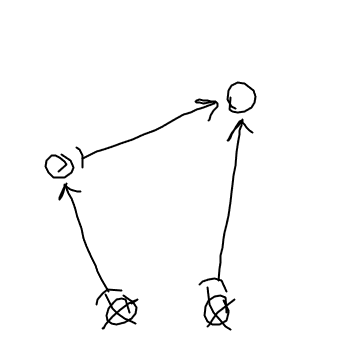
\includegraphics[width=\textwidth]{images/4bar_sketch.png}
        \caption{}
        \label{fig:4bar_sketch}
    \end{subfigure}
    \begin{subfigure}[b]{0.3\textwidth}
        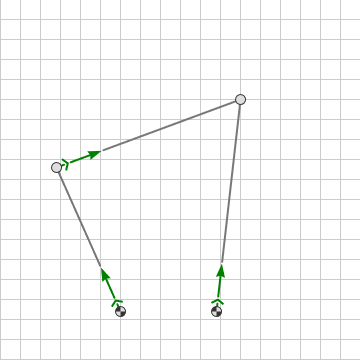
\includegraphics[width=\textwidth]{images/4bar_prediction.png}
        \caption{}
        \label{fig:4bar_prediction}
    \end{subfigure}
    \label{fig:4bar_example}
    \caption{Ein Viergelenk}
\end{figure}

\begin{figure}[H]
    \centering
    \begin{subfigure}[b]{0.3\textwidth}
        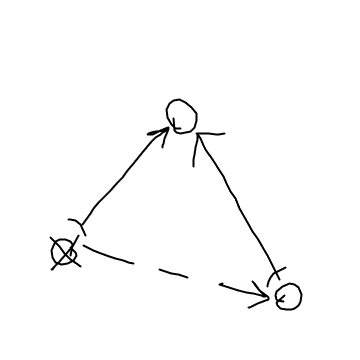
\includegraphics[width=\textwidth]{images/pump_sketch.png}
        \caption{}
        \label{fig:pump_sketch}
    \end{subfigure}
    \begin{subfigure}[b]{0.3\textwidth}
        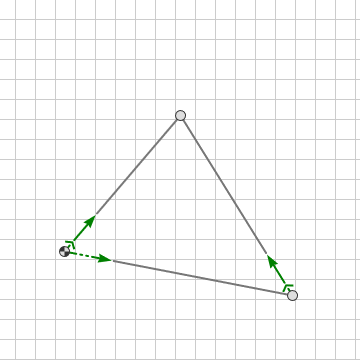
\includegraphics[width=\textwidth]{images/pump_prediction.png}
        \caption{}
        \label{fig:pump_prediction}
    \end{subfigure}
    \label{fig:pump_example}
    \caption{Mechanismus mit translatorischem Glied}
\end{figure}